\documentclass{article}[18pt]
\usepackage{../../../../format}
\lhead{Software Methodologies - Image Processing}


\begin{document}
\begin{center}
\underline{\huge Image Noise and Spatial Filtering I}
\end{center}
\section{Noise in images}
No digital image is a perfect representation of the original 2D signal\\
They are limited in resolution by sampling and contain noise\\
\\
Noise removal is a major goal of image processing to limit the effects on image visualisation and analysis
\section{Where does image noise come from?}
Capture:
\begin{itemize}
	\item Variations in sensor temperature
	\item Electrical sensor noise
	\item Sensor non-uniformity
	\item Dust in the environment
	\item Vibration
	\item Lens distortion
	\item Focus limitations
	\item Sensor saturation (too much light)
	\item Under exposure (too little light)
\end{itemize}
Sampling:
\begin{itemize}
	\item Limitations in sampling and intensity quantization (aliasing)
\end{itemize}
Processing:
\begin{itemize}
	\item Limitations in numerical precision
	\item Potential integer overflow
	\item Mathematical approximations
\end{itemize}
Image compression:
\begin{itemize}
	\item Lossy image compression techniques remove information from image to save space
	\item JPEG/MPEG are examples of widely used lossy compression formats
	\item Remove non-perceivable detail aiming at "no noticeable difference"
	\item Result: "compression artefacts" in the image
\end{itemize}
\section{Scene noise}
Lighting:\begin{itemize}
	\item Sunlight changes
	\item Varying artificial light sources
	\item Interior light sources oscillate with power supply frequency
	\item Objects cast shadows causing false image features
	\item As objects move shadows change
\end{itemize}
Occlusion:
\begin{itemize}
	\item Objects are frequently obscured by other objects: occlusion
	\item Big problem for recognition systems in image understanding tasks
\end{itemize}
\section{Types of theoretical noise models}
\subsection{Salt and pepper noise (impulse noise)}
\begin{itemize}
	\item Random white or black value pixels into the image
	\item Follows a binary high-low bi-modal noise distribution
\end{itemize}
\subsection{Gaussian noise (additive noise)}
\begin{itemize}
	\item Small random variation of the image signal around its true value following the Gaussian distribution
	\item This is the most common noise model in image processing
\end{itemize}
\section{Image noise removal}
\subsection{Neighbours of a pixel}
A pixel p at coordinates (x,y) has four horizontal and vertical neighbours whose coordinates are given by
$$(x+y,y), (x-1,y), (x,y+1), (x,y-1)$$
It also has four diagonal neighbours whose coordinates are given by:
$$(x+1,y+1),(x+1,y-1),(x-1,y+1),(x-1,y-1)$$
Together they form the $3\times 3$ local pixel neighbourhood\\
\\
Local image neighbourhoods define local areas of influence, relevance or interest\\
\\
Image filtering and many other operations use $N\times M$ neighbourhoods\\
\\
In most cases:
\begin{itemize}
	\item N=M (we treat both directions equally)
	\item N is odd (simplifies implementation)
\end{itemize}
\section{Spatial filtering}
We go iteratively through the pixels we want to process (perhaps the whole image)\\
\\
for each pixel (i,j):
\begin{itemize}
	\item Consider a neighbourhood S of (i,j). Usually (i,j) will be at the centre of S
	\item Process the pixel values of S (i.e. apply to them a many to one function) to find a new value for pixel (i,j)
\end{itemize}
Replace the original pixel values with the new ones (called the filter's responses)
\begin{center}
	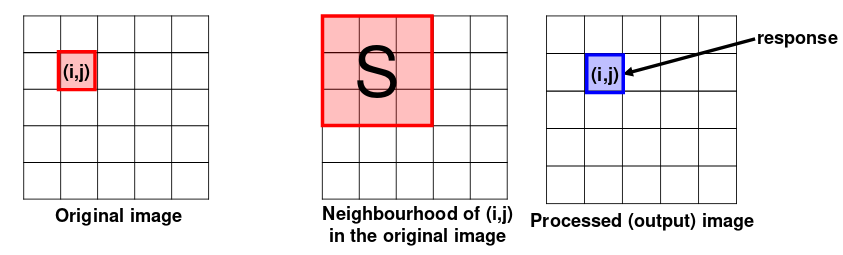
\includegraphics[scale=0.7]{neighbourhood}
\end{center}
\section{Filtering}
\begin{defin}[Linear filtering]
Output pixel is a linear combination of the corresponding input pixel's neighbourhood
\end{defin}
\begin{defin}[Non-linear filtering]
Output pixel is not linear function of the corresponding input pixel's neighbourhood. In practice, some decision based algorithm is employed
\end{defin}
\section{Mean filter}
\textbf{Operation}: Replace a given pixel with the mean (unweighed average) of its $N\times N$ image neighbourhood
\[
I_{o u t p u t}(i, j)=\frac{1}{N^{2}} \sum_{(i, j) \in S} I_{i n p u t}(i, j)
\]
S is the neighbourhood, a rectangular window centred at pixel (i,j) enclosing $N\times N$ neighbours\\
\\
\textbf{Effect}: Eliminates sudden intensity jumps which could be caused by some noise processes, i.e. eliminates large deviations from the norm.
\subsection{Example}
Suppose we have the $3\times 3$ neighbourhood:
\[
\begin{array}{lll}{2} & {2} & {3} \\ {3} & {30} & {2} \\ {1} & {3} & {2}\end{array}
\]
Thee value 30 is relatively large - noise spike\\
\\
Mean filtering will suppress it:
\[
\begin{array}{lll}{2} & {2} & {3} \\ {3} & {5.3} & {2} \\ {1} & {3} & {2}\end{array}
\]
\subsection{Effect on types of noise}
\textbf{Gaussian noise}: Distributed around the original value - the mean can easily handle this\\
\textbf{Salt and pepper noise}: Significant deviation from the local distribution
\subsection{Drawbacks}
Mean filter is not robust to large noise deviations (statistical outliers). For example, a single pixel with a very unrepresentative value.\\
\\
Mean filter causes edge blurring, that is, removes the high frequency sharp detail.
\section{Spatial non-linear filters}
For an $N\times N$ image neighbourhood, $N_{xy}$, centred at pixel (x,y)  and index by (s,t) the following simple statistical filters can be defined to replace each pixel with the min/max/median from the input neighbourhood\\
\\
Min:
\[
\min _{(s, t) \in N_{x y}}\left\{I_{i n p u t}(s, t)\right\}
\]
Max:
\[
\max _{(s, t) \in N_{x y}}\left\{I_{\text {input}}(s, t)\right\}
\]
Median:
\[
\operatorname{median}_{(s, t) \in N_{x y}}\left\{I_{i n p u t}(s, t)\right\}
\]
\subsection{Other spatial non-linear filters}
Alpha tripped mean:
\[
I_{o u t p u t}(x, y)=\frac{1}{N^{2}-2 d} \sum_{(s, t) \in N_{x y}} I_{\text {Input}_r}(s, t)
\]
Here, the dimension of the neighbourhood $N_{xy}$ is $N\times N$. The d lowest and the d highest intensity levels of the image in $N_{xy}$ are deleted (set to 0) with $I_{Input_r}(s,t)$ denoting the remaining (reduced set of) $N^2-d$ pixels in $N_{xy}$\\
\\
Harmonic mean:
{\Large
\[
I_{o u t p u t}(x, y)=\frac{N^{2}}{\sum_{(s, t) \in N _{x y}} \frac{1}{I_{i n p u t}(s, t)}}
\]
}
\section{Median Filter}
\textbf{Operation}: Replace a given pixel with the median of its $N\times N$ image neighbourhood\\
\\
Example: for $3\times 3$
\begin{center}
	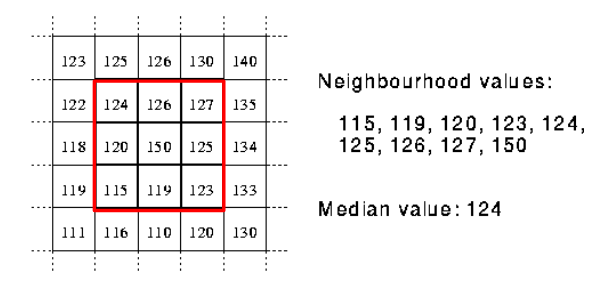
\includegraphics[scale=0.7]{Median}
\end{center}
\textbf{Effect}: Eliminates sudden intensity jumps which could be caused by some noise processes, i.e. large deviations from the norm.\\
\\
But, it is robust to statistical outliers (unlike the mean filter)\\
\\
\textbf{Example}: Suppose we have the $3\times 3$ neighbourhood:
\[
\begin{array}{lll}{2} & {6} & {3} \\ {14} & {81} & {2} \\ {13} & {4} & {1}\end{array}
\]
The value 81 is relatively large - noise spike (an outlier)\\
\\
Median filtering will suppress it
\[
\begin{array}{lll}{2} & {6} & {3} \\ {14} & {4} & {2} \\ {13} & {4} & {1}\end{array}
\]
\section{Conservative smoothing}
\textbf{Operation}: Compare a pixel value to min and max of the other ($N\times N -1$) neighbourhood pixels:
\begin{itemize}
	\item Replace by min if $<$ min
	\item Replace by max if $>$ max
\end{itemize}
Example: For $N=3$
\begin{center}
	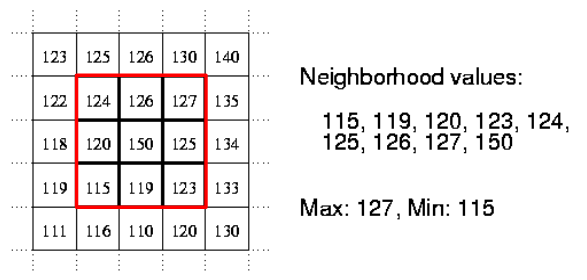
\includegraphics[scale=0.7]{Smoothing}
\end{center}
\textbf{Effect}: Eliminates sudden intensity jumps\\
\\
Here, 150 is replaced by 127 (max of its 8 neighbours)\\
\\
A conservative approach to smoothing:
\begin{itemize}
	\item A pixel value will change only if it is outside the range of its neighbours
	\item By the minimum required amount to just bring it in to range
\end{itemize}
\end{document}
